\section{Ristrutturazione del modello concettuale}
\subsection{Analisi delle ridondanze}
È presente una ridondanza nel campo \textit{hire\_date} di \textit{base\_emp} in quanto è possibile calcolarla dall'entità associata \textit{career\_log}
\subsection{Eliminazione degli attributi multivalore}
Non sono presenti attributi multivalore
\subsection{Eliminazione degli attributi composti}
L'attributo \textit{address} di \textit{site} è un attributo composto.

Siccome l'indirizzo è unico per ogni sede, si è deciso di accorpare gli attributi di \textit{address} in \textit{site}.\meskip
L'attributo \textit{tech\_specs} di \textit{equipment} potrebbe essere scomposto in più attributi ma in questo caso non è necessario ai fini della traccia, quindi è più comodo memorizzarlo come un unico campo stringa.

\subsection{Analisi delle generalizzazioni}
Procediamo all'eliminazione delle generalizzazioni partendo dal basso:
\begin{enumerate}
	\item Accorpamento di \textit{scientific\_referent} e \textit{scientific\_manager} in \textit{senior} in quanto non avendo attributi non è possibile inserire valori nulli che occupano spazio inutile.\\
	      Fatta tale scelta bisogna cambiare la cardinalità da $\;(1, n)\;$ a $\;(0, n)\;$ in entrambe le associazioni, poiché un \textit{senior} può anche non essere nessuno dei due o uno soltanto (overlapping parziale)
	\item Accorpamento di \textit{junior}, \textit{middle}, \textit{senior}, \textit{manager} all'interno di \textit{base\_emp} aggiungendo un attributo che ne specifica il tipo.\\
	      Notare che questa scelta aggiunge una \textbf{ridondanza} poiché il tipo è reperibile effettuando un'interrogazione in \textit{career\_log}. Nonostante ciò è più efficiente e immediato eseguire determinate operazioni avendo quest'attributo disponibile direttamente in \textit{base\_emp}
	\item Accorpamento di \textit{employee} all'interno di \textit{project\_salaried} e \textit{base\_emp} in quanto la generalizzazione è totale.
\end{enumerate}
\subsection{Identificazioni chiavi primarie}
\begin{itemize}
	\item In \textit{base\_emp} abbiamo l'attributo \textit{CF} (Codice Fiscale), una stringa di $16$ caratteri
	\item In \textit{project\_salaried} abbiamo l'attributo \textit{CF} (Codice Fiscale), una stringa di $16$ caratteri
	\item \textit{project} è identificato dal \textit{CUP} (Codice Univoco Progetto)
	\item \textit{equipment} è identificato da \textit{code} che è un codice generato randomicamente
	\item \textit{equipment\_request} è identificato da \textit{code} che è un codice generato randomicamente
	\item \textit{site} è identificato da un nuovo attributo \textit{site\_number} che si autoincrementa
	\item \textit{laboratory} è identificato da un nuovo attributo \textit{lab\_code} che si autoincrementa
\end{itemize}
\newpage

\subsection{Schema ristrutturato UML}
\bigskip 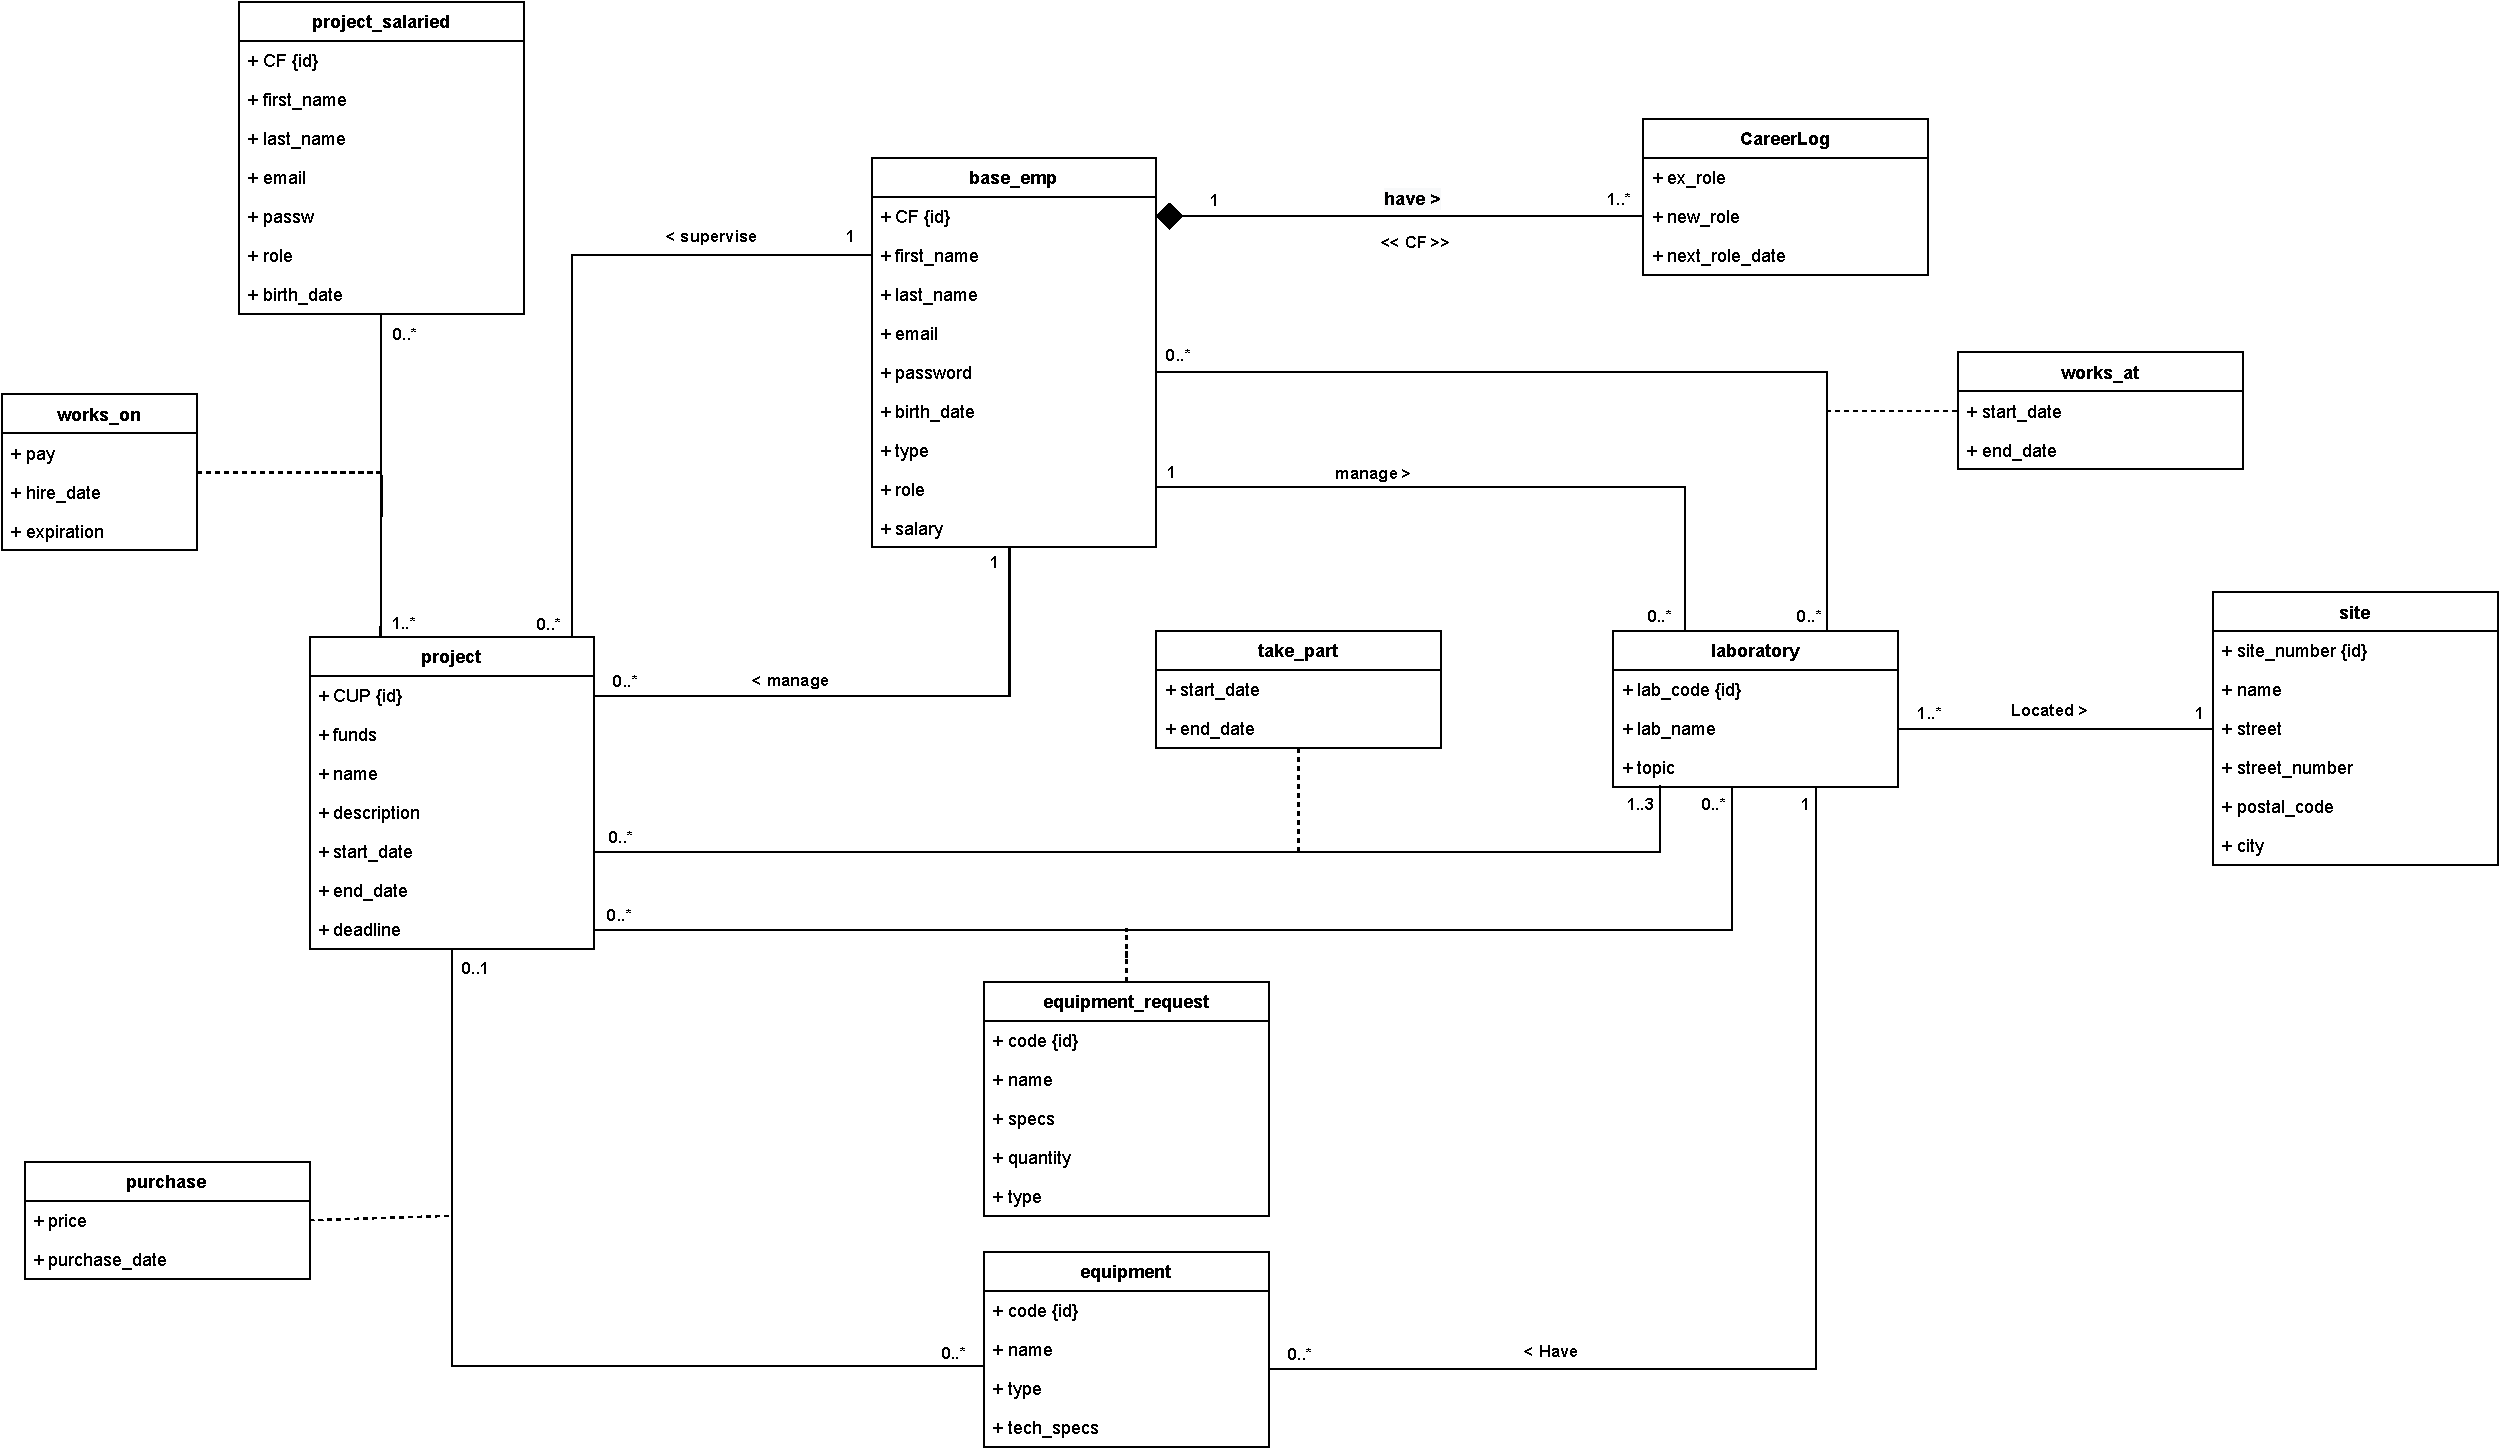
\includegraphics[width=\textwidth]{images/Ristrutturato-UML.drawio.pdf}


\subsection{Schema ristrutturato ER}
\bigskip 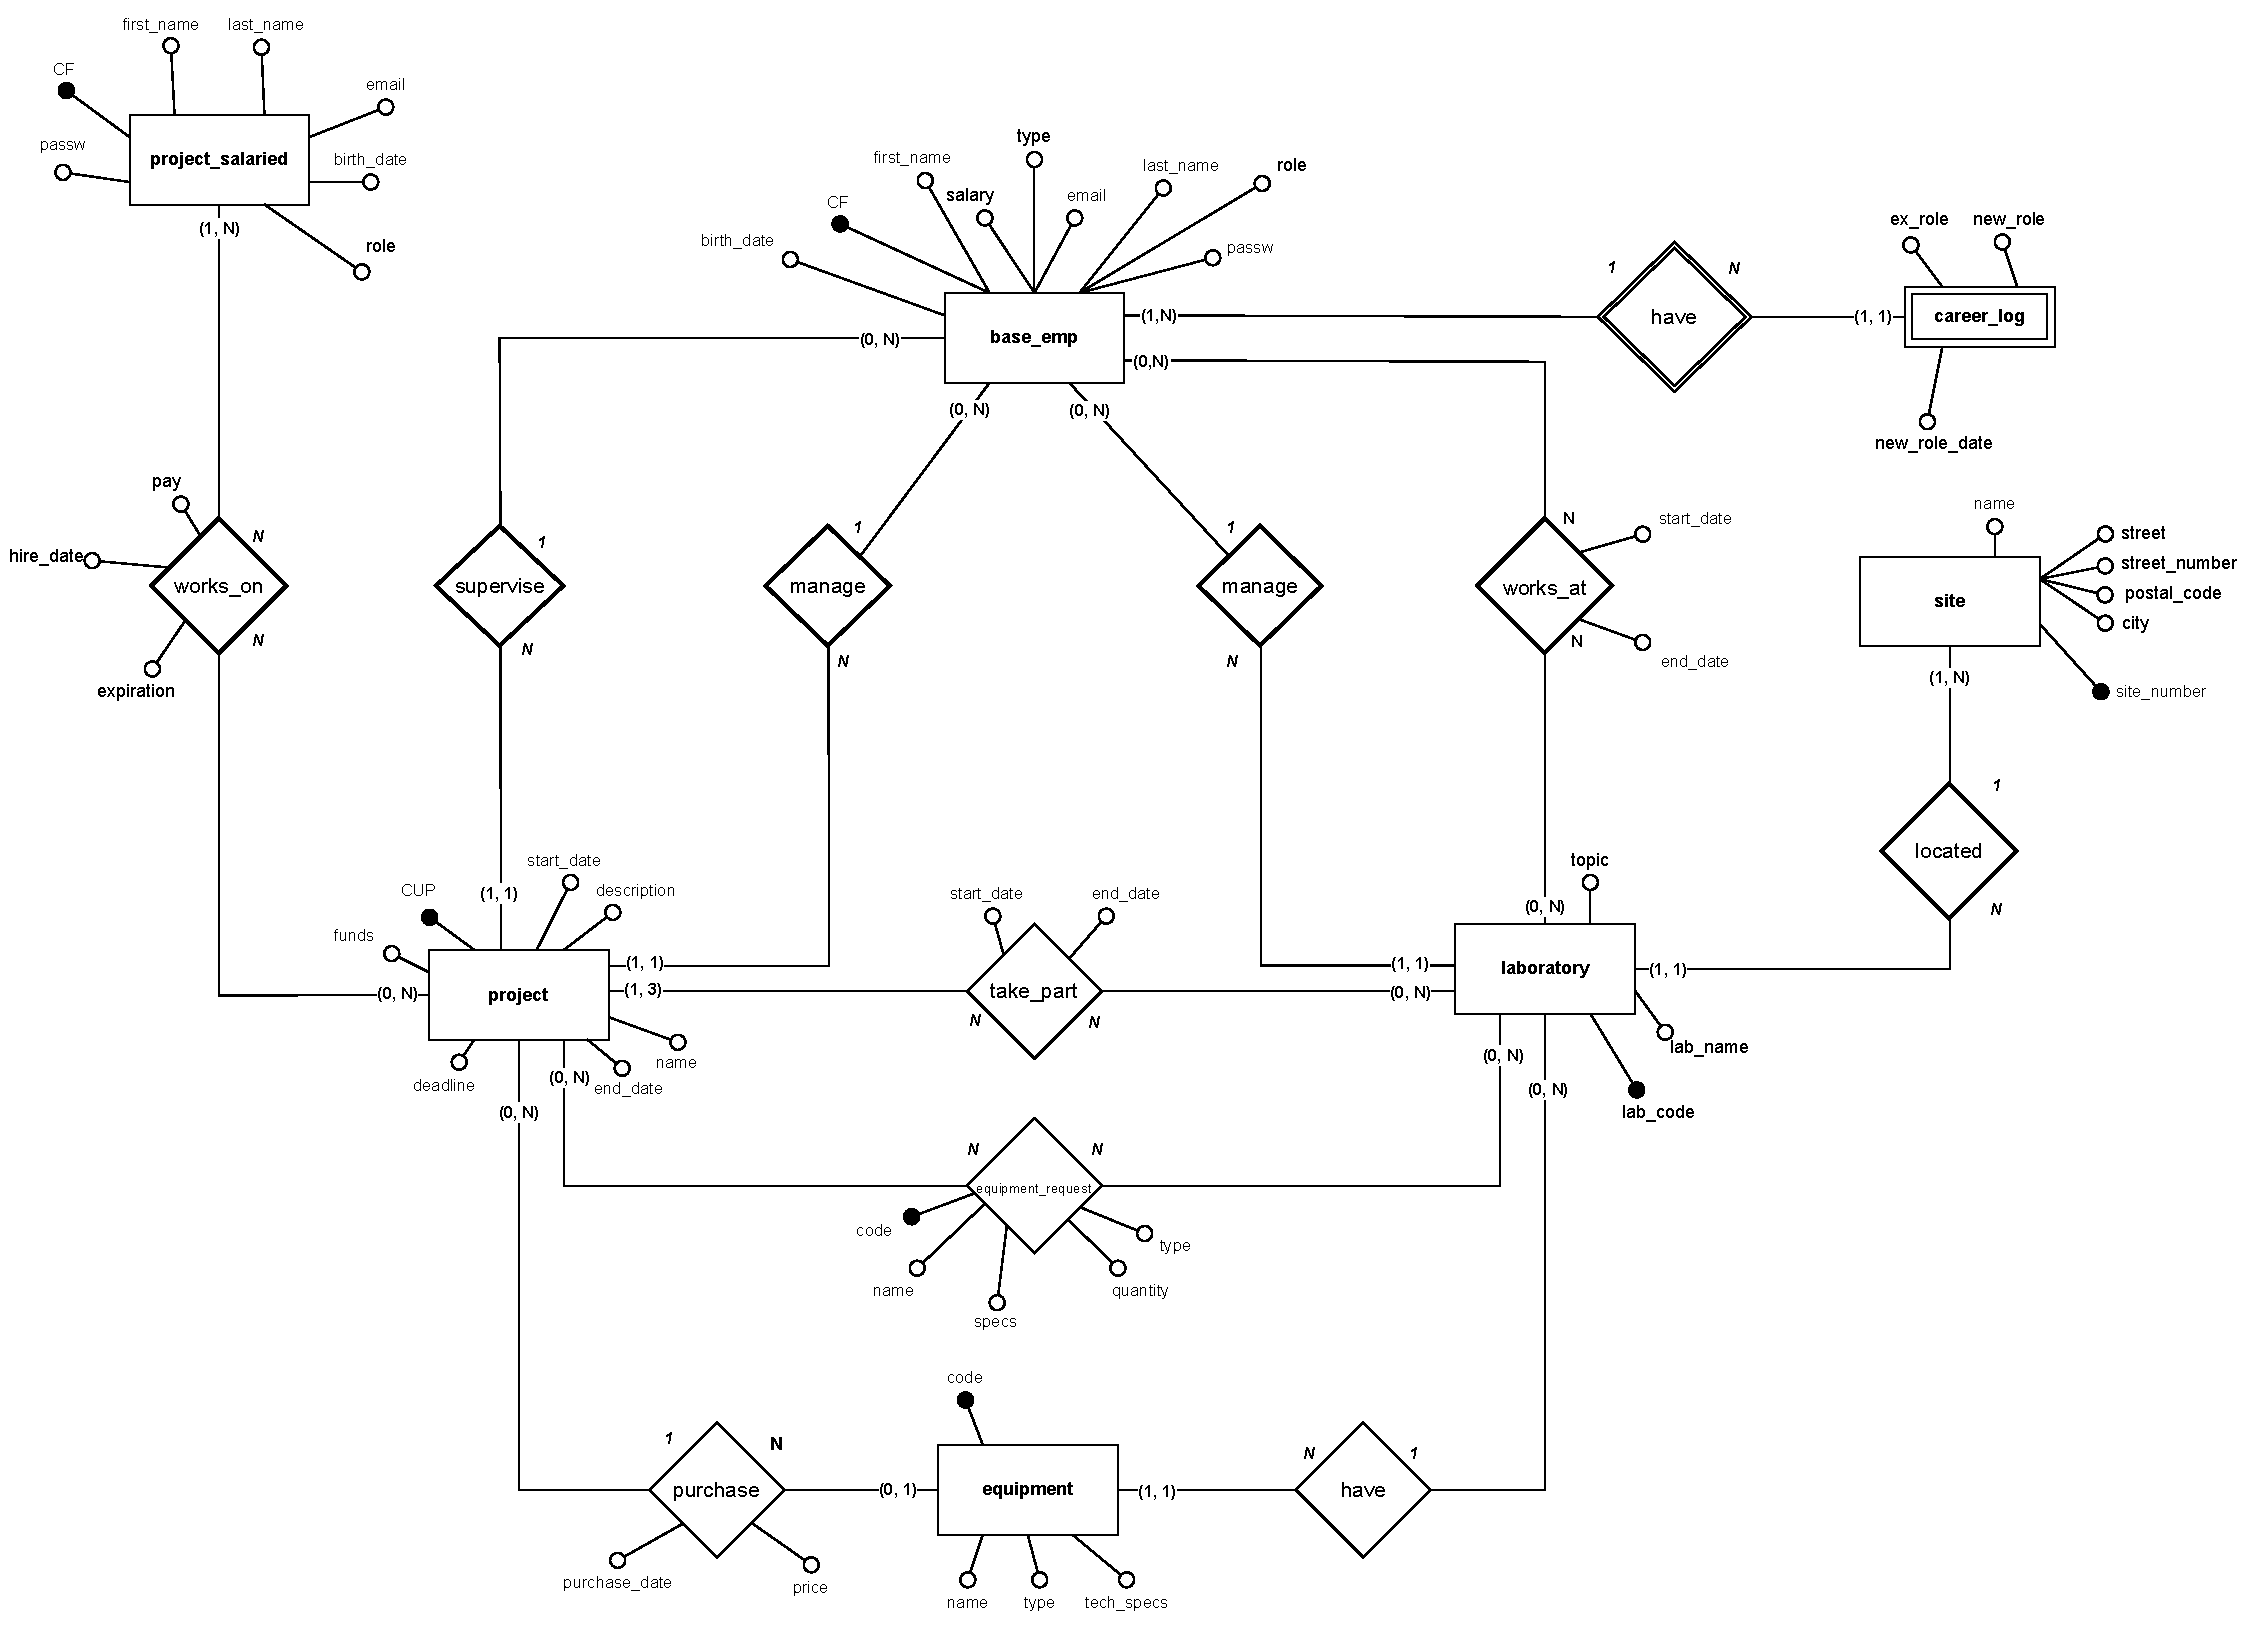
\includegraphics[width=\textwidth]{images/Ristrutturato-ER.drawio.pdf}



